% !TEX program = xelatex

% Základní balíčky
\documentclass[10pt,a4paper]{article}
\usepackage[utf8]{inputenc}
\usepackage[T1]{fontenc}
\usepackage{graphicx}
\usepackage{calc}
\usepackage[top = 1cm, bottom = 1cm, left = 1cm, right = 1cm]{geometry}


% Matematika
\usepackage{amsmath}
\usepackage{amssymb}
\usepackage{mathtools}
\usepackage{nicefrac}
\usepackage{gensymb}

% MISC
\usepackage{hyperref}
\usepackage{listings}
\usepackage{multirow}

% Jazyky
\usepackage[czech]{babel}
\AtBeginDocument{\shorthandoff{-}} % český Babel rozbíjí jiné balíčky, tohle je fix
\usepackage{csquotes}
\usepackage{polyglossia}
\setmainlanguage{czech}
\setotherlanguage{greek} % aby se dalo psát αβγδ... do textu

% Pro titulní stránku
\usepackage{titlesec}
\usepackage{setspace}
\usepackage{framed}
\usepackage{array}

% Grafy
\usepackage{gnuplottex}
\usepackage{epstopdf}

% Pokročilé figures
\usepackage{wrapfig}
\usepackage{nonfloat}

% Načítání tabulek z CSV
\usepackage{csvsimple}

% více obrázků v jednom Fig.
\usepackage{subfig}

% přidávání stránek z PDF do dokumentu
\usepackage{pdfpages}

% přeškrtnutý text pomocí \st
\usepackage{soul}


% z rodiny \phantom, \vphantom a \hphantom
% \mask{A}{B} udělá mezeru o šířce A a doprostřed napíše B
\newcommand*{\mask}[2]{\mathord{\makebox[\widthof{\(#1\)}]{\(#2\)}}}

% na sázení jednotek
\renewcommand{\U}[1]{\ensuremath{\,\mathrm{#1}}}
\newcommand{\°}{\degree}


% pro titulku
\newcommand{\titjmeno}{Michal Grňo}
\newcommand{\titobor}{FOF}
\newcommand{\titcislo}{A69}
\newcommand{\titnazev}{Měření toho a toho}
\newcommand{\titmereni}{1. 1. 1900}
\newcommand{\titodevzdani}{1. 1. 2000}




\begin{document}


\thispagestyle{empty}
\newgeometry{top = 2.5cm, bottom = 0cm, left = 2.5cm, right = 3cm}

{%T tomto je uzavřena celá titulka
%Tloušťka rámečku
\setlength{\fboxrule}{1.5pt}

\noindent
\framebox{
\begin{minipage}{\textwidth}
\setlength{\parindent}{17.62482 pt}
\phantom{d}

\begin{minipage}{0.6\textwidth}
{
\Large Kabinet výuky obecné fyziky, UK MFF\\
}
\vspace*{0.2cm}

{
\bfseries
\huge Fyzikální praktikum %ČÍSLO
}
\end{minipage}
\begin{minipage}{0.4\textwidth}
\begin{center}
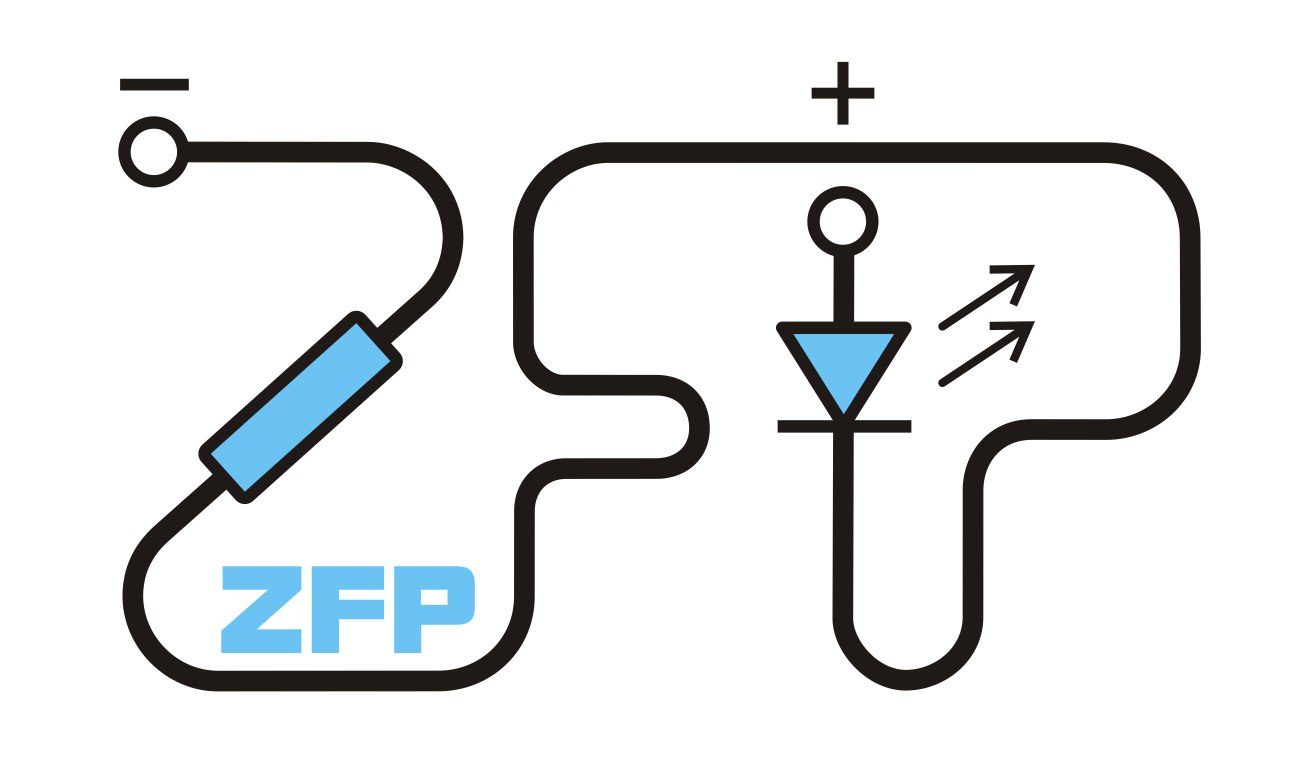
\includegraphics[width=4.5cm]{ZFP.jpg}
\end{center}
\end{minipage}\\\\

%\vspace*{0.5cm}

{
\setstretch{1.5}
\Large
\noindent
Úloha č. \titcislo

\noindent
Název úlohy: \titnazev

\noindent
Jméno: \titjmeno
\hspace*{\fill}
Obor: \titobor

\noindent
Datum měření: \titmereni
\hspace*{\fill}
Datum odevzdání: \titodevzdani

\phantom{d}
}
\end{minipage}
}
%Konec horního rámečku

{
\phantom{d}

\Large
Připomínky opravujícího:\\
\vspace*{6.75cm}
}

\newcommand{\linka}{\noalign{\hrule height 1pt}}
\newcommand{\linkadva}{\noalign{\hrule height 1.5pt}}
\setlength\extrarowheight{9.5pt}
\Large
\noindent
\begin{tabular}{!{\vrule width 1.5pt} l !{\vrule width 1pt} c !{\vrule width 1pt} c !{\vrule width 1.5pt}}
\linkadva
   & Možný počet bodů & Udělený počet bodů \\\linkadva
  Práce při měření & 0-3 &  \\\linka
  Teoretická část & 0-2 &  \\\linka
  Výsledky a zpracování měření & 0-9 &  \\\linka
  Diskuse výsledků & 0-4 &  \\\linka
  Závěr & 0-1 &  \\\linka
  Použitá literatura & 0-1 &  \\\linkadva
  \hspace*{\fill} \textbf{Celkem} \hspace*{\fill}& max. 20 &  \\
\linkadva
\end{tabular}
\phantom{d}

Posuzoval: \hspace*{\fill}dne:~~~~~~~~~~~~~~~~~

}%Konec uzavření titulky
\newpage
\newgeometry{top = 2cm, bottom = 2cm, left = 2cm, right = 2cm}
\setcounter{page}{1}

\setmainfont{Linux Libertine O}


\section{Pracovní úkoly}
\begin{enumerate}
    \item První úkol
    \item Druhý úkol
\end{enumerate}

\section{Teoretická část}
Budeme měřit veličinu $\alpha$, pro kterou platí vzorec
\begin{equation}
    \alpha = \frac{ 0.5 \, \alpha^3 }{ \alpha^2 / 2 } \: .
    \label{eq-alpha}
\end{equation}
Další význačná veličina je \textit{rapidita} $\beta$, která je definovaná jako: [1]
\begin{equation*}
    \beta = \nicefrac{\displaystyle v}{\displaystyle c} \: ,
\end{equation*}
kde $v$ je rychlost objektu a $c$ je rychlost světla.

\pagebreak

\section{Měření a zpracování dat}
Naměřili jsme tabulku čísel:
\begin{table}[h!]
    \centering
    \begin{tabular}{ c|c }
        $\alpha$ & $\beta$ \\\hline
        \csvreader[ head to column names ]{tabulka-data.csv}{}
        {
            \csviffirstrow{}{\\}
            \dataAlpha & \dataBeta
        }
    \end{tabular}
    \caption{}
    \label{}
\end{table}


\begin{figure}[t]
    \centering
    % zkompilujeme příkazem "make gnuplot"
    \begin{gnuplot}[terminal=epslatex,terminaloptions={color size 15cm, 8cm}]
        set key top left
        set xlabel '$\alpha$'
        set ylabel '$\beta$'

        set datafile separator ','

        a = b = 1
        f(x) = a*x + b

        fit f(x) 'tabulka-data.csv' skip 1 via a, b


        set xrange [0:100]
        set yrange [0:500]

        plot 'tabulka-data.csv' skip 1 t 'Naměřená data', f(x) t 'Lineární regrese'
    \end{gnuplot}
    \caption{Výstup z transgresního žouželátoru.}
    \label{img-kalibrace}
\end{figure}

Ke zpracování jsme použili Python:
\lstinputlisting[language=Octave]{./kod.py}
Naměřená data jsme potom vynesli do grafu v obrázku č. \ref{img-kalibrace}.


\section{Diskuse}
Vyšlo to jinak než na Brejlovci, takže jsme asi něco zanedbali. (Možná teplotní roztažnost židle, na které seděl experimentátor?)

\section{Závěr}
Bylo to krásné.

\section{Literatura}
[1] Praktikum částicové a jaderné fyziky. Zeemanův jev. 2002. \\ Dostupné z: \url{https://physics.mff.cuni.cz/vyuka/zfp/_media/zadani/texty/txt_417.pdf}.
\\[10pt]

\end{document}
